\chapter{Implementation}
\label{cha:implementation}

\section{Scripts for data analysis - usage}

TODO: 

\section{Stop Location Identification - batch processing in Apache Spark}

TODO: final implementation and algorithm should be discussed here

\subsection{Calculation of the index for verification of mobility index approach - python implementation}

There are two approaches to calculate mobility index, having equally spaced windows in time, or sliding window.
\\\\
In the first approach, for a single user, minimum and maximum timestamp of sorted sequence is being found. Having value of MobilityIndexWindow (e.g. 30 minutes), function is creating equaly spaced bins of that value within maximum and minimum timestamps. Each point is being visited and is assigned to the proper timestamp bin according to its own timestamp and duration to the previous point. 
\\\\
In the second approach, for a single user, each point is being visited and temporarly marked as "current position". For each current position, all points which are distant in time by MobilityIndexWindow in the past, are assigned to the sliding window.

\begin{figure}
	\centering
	\begin{minipage}{.5\textwidth}
		\centering
		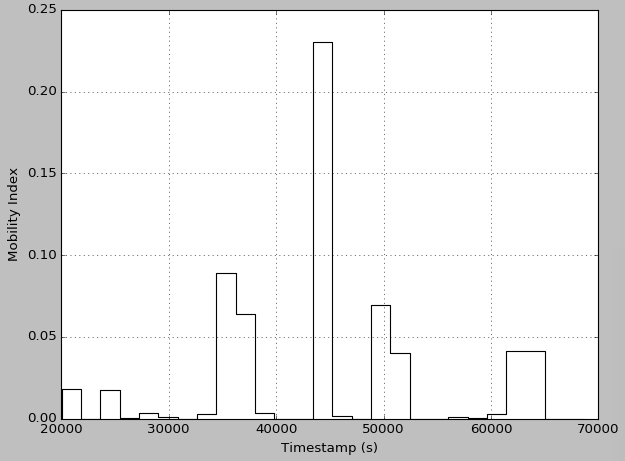
\includegraphics[width=.9\linewidth]{images/mob_calc1.png}
	\end{minipage}%
	\begin{minipage}{.5\textwidth}
		\centering
		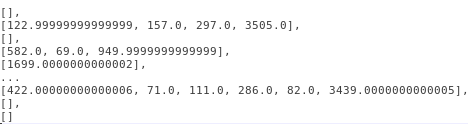
\includegraphics[width=.9\linewidth]{images/mob_calc2.png}
	\end{minipage}
	\captionof{figure}{Mobility Index calculation using equally spaced windows in time (left) and using sliding window over time (right). Time Window of 30 minutes using the same data set for one unique user}
	\label{fig:mob_calc}
\end{figure}

\FloatBarrier

At the end, mobility index, as defined in \autoref{cha:introduction_mob_index_sect}, is being calculated over the assigned values - \autoref{fig:mob_calc}. 

\subsection{Algorithm for stop detection}

TODO

\section{Clustering algorithm}

For clustering we started off with DBScan, described in \autoref{chap:related_work}. The difficulty with DBScan is figuring out the two parameters, the minimum points per cluster (\textit{minPts}) and the radius of the clusters (\textit{eps}). 

\subsection{DBSCAN on Spark}

We wanted a scalable implementation of DBSCAN that could handle large data sets, preferable in parallel. We decided to use Apache Spark, a scalable engine for large-scale data processing \cite{spark}. For this we used an implementation by Irving Cordova, based upon an algorithm called MR-DBSCAN built for the MapReduce framework \cite{dbscan_on_spark}. The implementation of DBScan runs in parallel by splitting the data space into boxes, using the number of boxes as a cost estimator for the algorithm. Each box then grows to include one \textit{eps} in it. After each box and its points has been determined the traditional DBScan algorithm is run on the points in each box. Finally it examines the intersection points betweeen boxes and merges the result together \cite{vis_dbscan_on_spark}. The figures below visualises the execution steps.

\begin{figure}
	\centering
	\begin{minipage}{.5\textwidth}
		\centering
		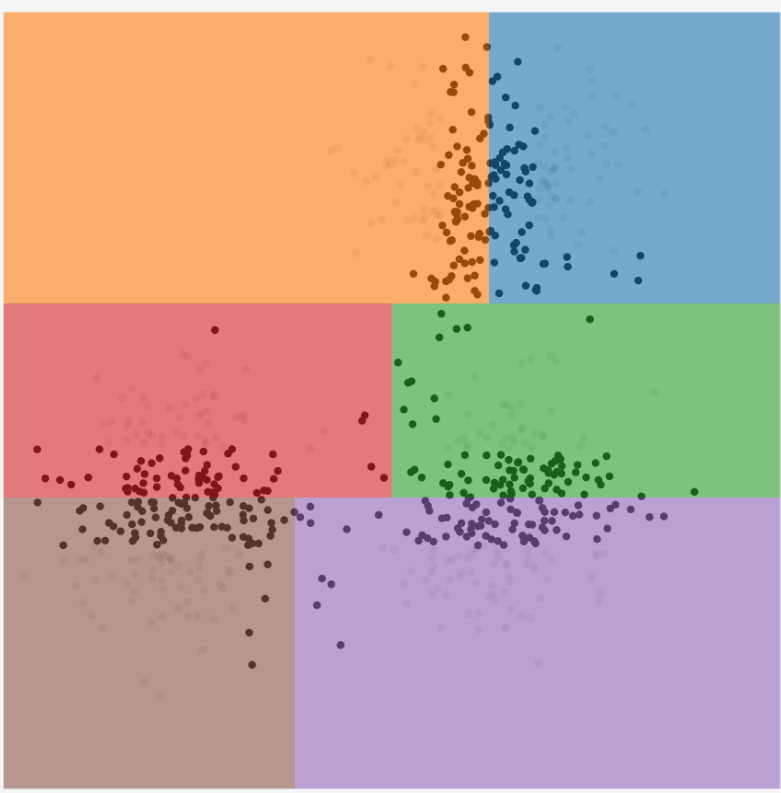
\includegraphics[width=.6\linewidth]{images/db1_c.png}
		\captionof{figure}{Step 1. DBSCAN on Spark assign the data space into boxes.}
		\label{fig:db1_c}
	\end{minipage}%
	\begin{minipage}{.5\textwidth}
		\centering
		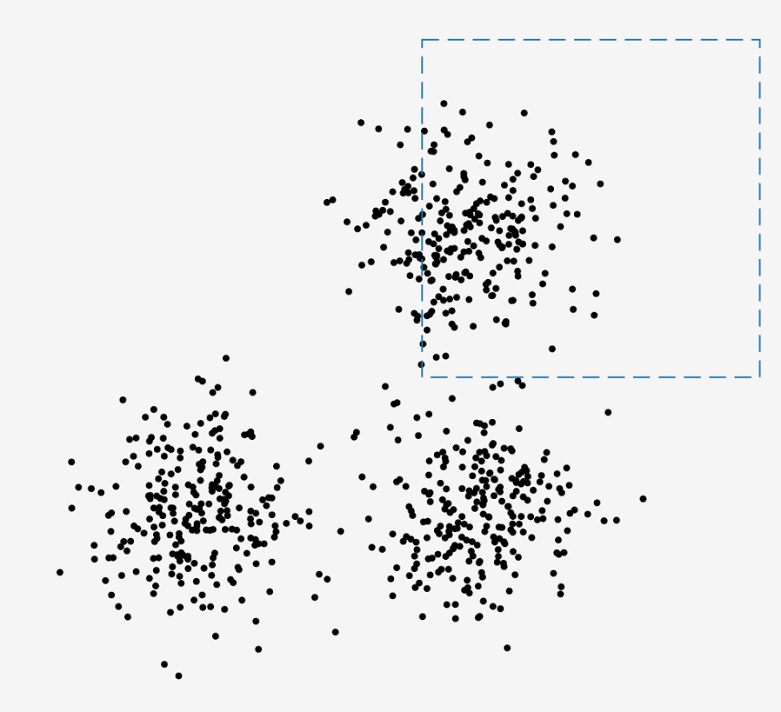
\includegraphics[width=.6\linewidth]{images/db2_c.png}
		\captionof{figure}{Step 2. Each box grows to include the points that are within one \textit{eps} of it.}
		\label{fig:db2_c}
	\end{minipage}
	\begin{minipage}{.5\textwidth}
		\centering
		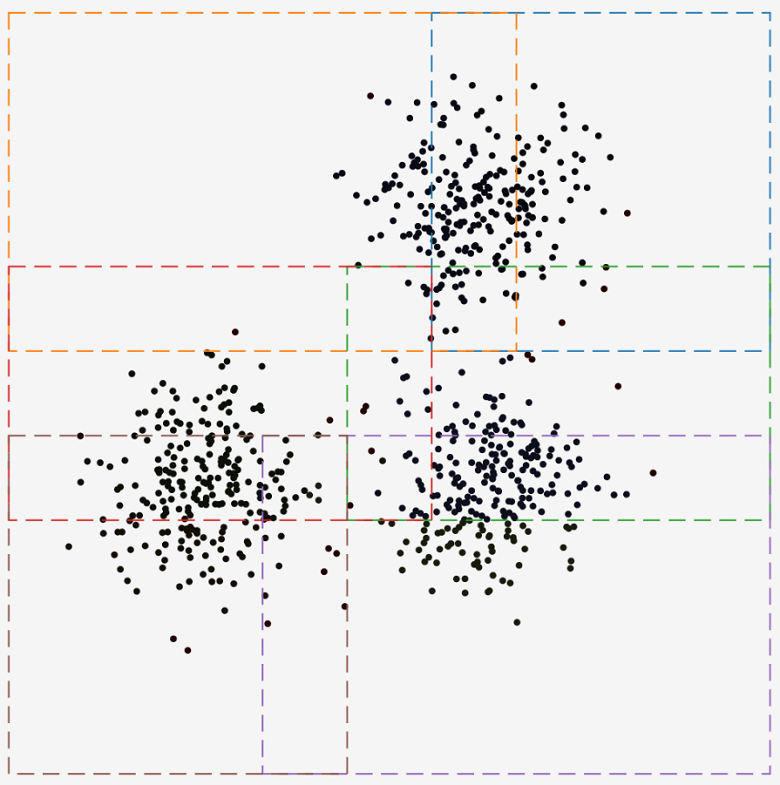
\includegraphics[width=.6\linewidth]{images/db3_c.png}
		\captionof{figure}{Step 3. Traditional DBScan algorithm is applied in parallel for each box. Each different color represents a different cluster. }
		\label{fig:db3_c}
	\end{minipage}%	
	\begin{minipage}{.5\textwidth}
		\centering
		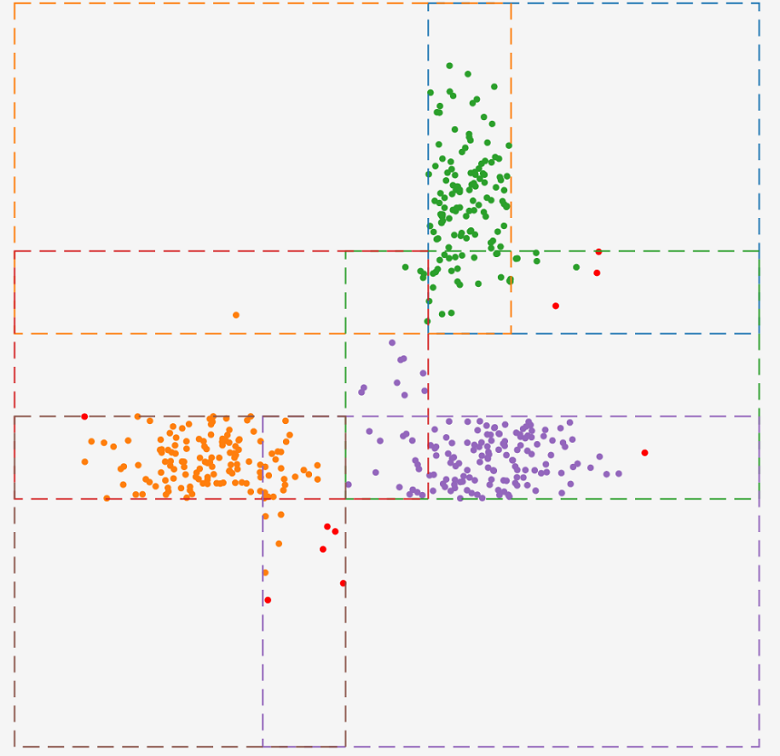
\includegraphics[width=.6\linewidth]{images/db4_c.png}
		\captionof{figure}{Step 4. After DBSCAN is done, all points witihin the borders of two clusters are examnied. If they are part of a cluster within two boxes they are merged to one cluster. }
		\label{fig:db4_c}	
	\end{minipage}		
	\begin{minipage}{.5\textwidth}
		\centering
		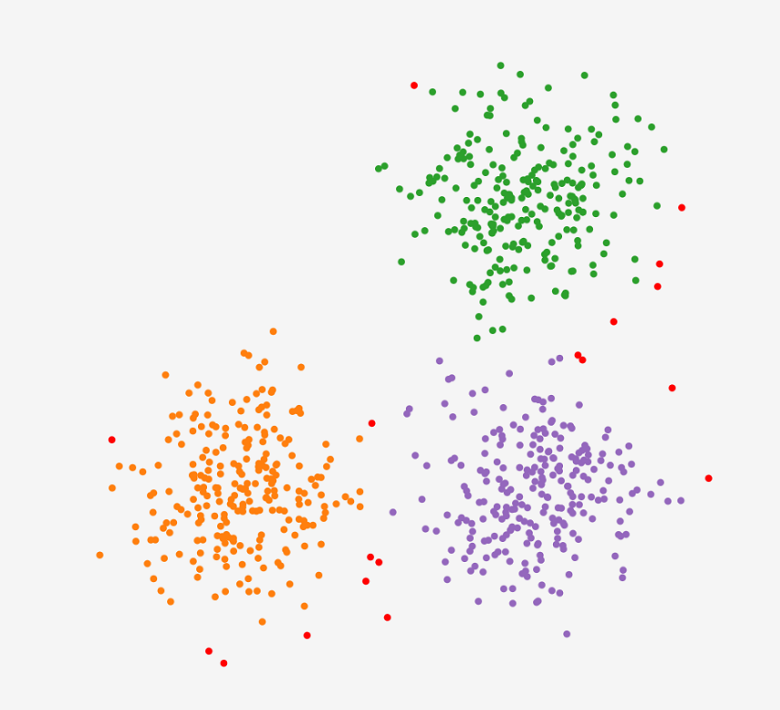
\includegraphics[width=1\linewidth]{images/db5_c.png}
		\captionof{figure}{Step 5. Finally all remaning points are labeled with the global identified cluster and we are done. (red points are noise points). }
		\label{fig:db5_c}	
	\end{minipage}%
\end{figure}






